\section{Sensitivity Analysis}
\label{a:sensitivity-analysis}

Twice during the process sensitivity analysis was performed. Both were carried out by performing a feature scoring analysis. Feature scoring was chosen, as also described in section \ref{ss:sensitivity-analysis}, because while still using the SOBOL sampling method, it has lower computational requirements \cite{jaxa-rozen_tree-based_2018}.
Figure~\ref{fig:msmordm} shows sensitivity analysis was employed to look at the model without any policies in place, and to look at the effect of the uncertainties on the policies. The results from this can be seen in figures \ref{fig:feat-scor-g-wo} - \ref{fig:feat-scor-o-wo} (sensitivity analysis without policies) and figures  \ref{fig:feat-scor-g} - \ref{fig:feat-scor-o} (sensitivity analysis with policies) below. Since the costs only regard the costs of implementing policies, all costs for the sensitivity analysis without policies were 0, hence its omission from the graphs. Since the levers for all actors were off, all these levers have an estimator value of 0. The levers for Deventer's dike are not included in their sensitivity analysis, as that is not a lever for them. 

We opted to combine the results from the sensitivity analysis per policy, as all experiments proved to be sensitive to the same uncertainties (just to a different extent). Even with RfR-projects in place, A.4\_pfail, the durability of Gorssel's dike, and A.5\_pfail, the durability of Deventer's dike, are the most dominant uncertainties.

\begin{figure}[h!]
    \centering
    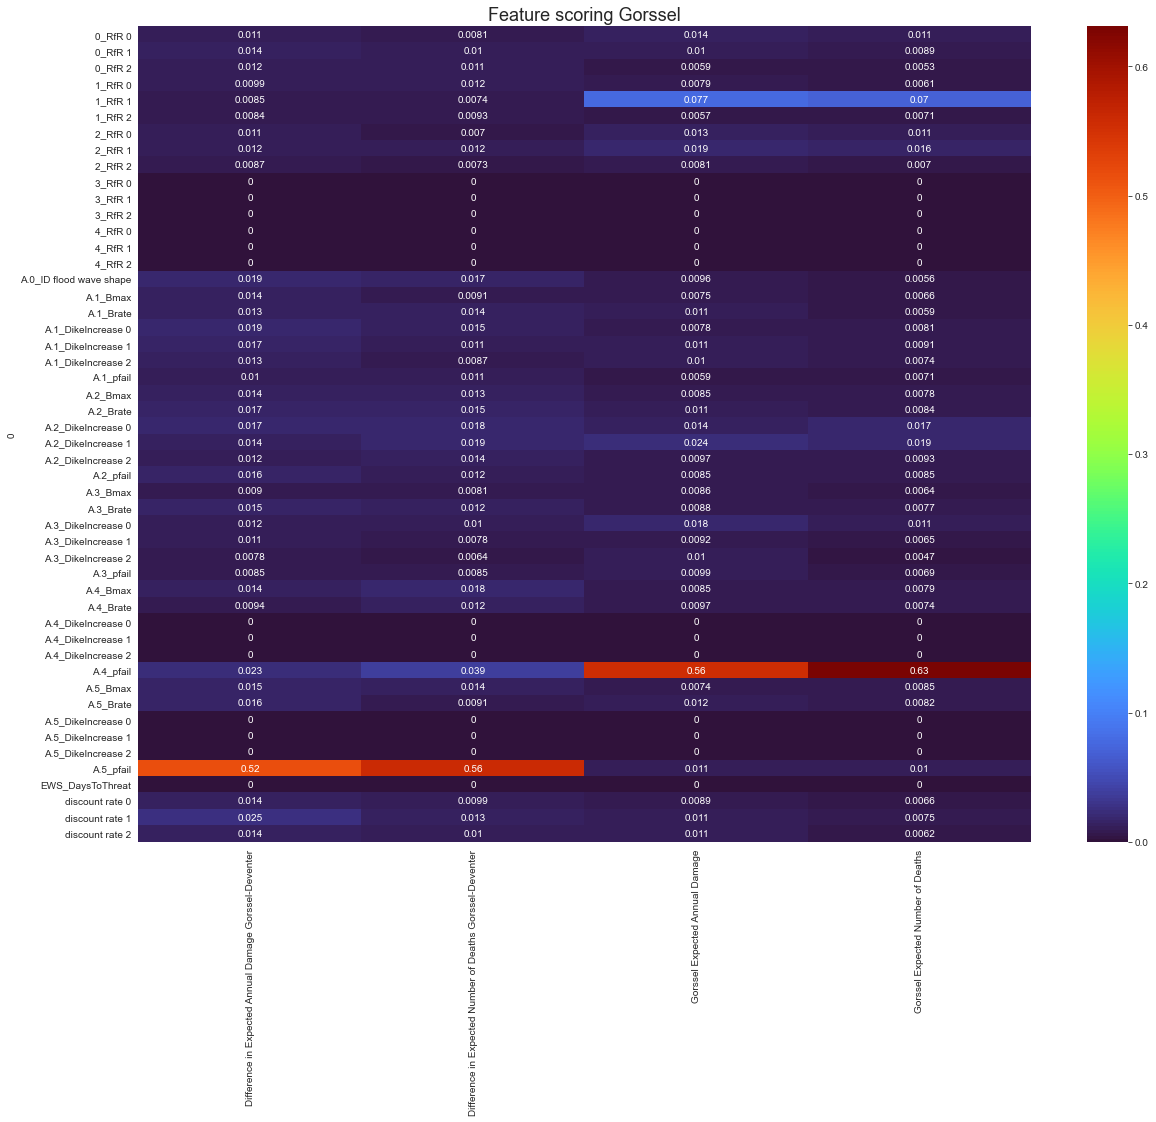
\includegraphics[width=\textwidth]{report/figures/results/sa_model_Gorssel.png}
    \caption{The results from feature scoring for the sensitivity analysis of Gorssel without policies.}
    \label{fig:feat-scor-g-wo}
\end{figure}

\begin{figure}[h!]
    \centering
    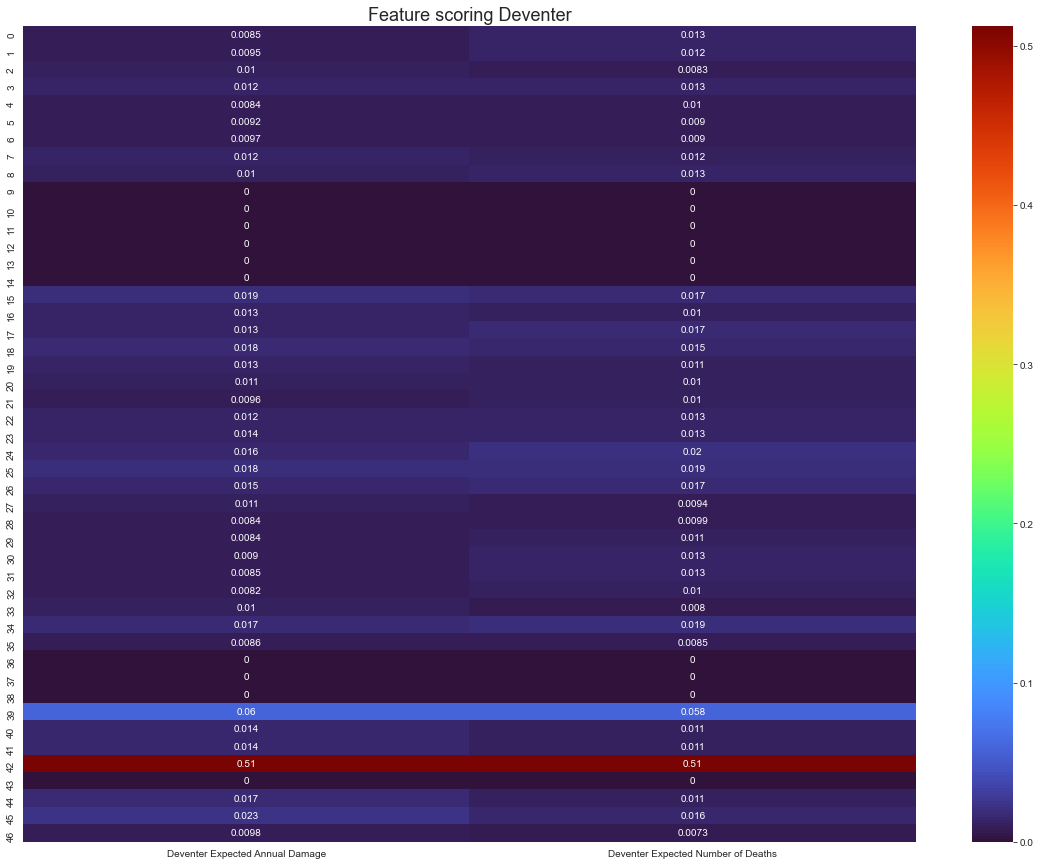
\includegraphics[width=\textwidth]{report/figures/results/sa_model_Deventer.png}
    \caption{The results from feature scoring for the sensitivity analysis of Deventer without policies.}
    \label{fig:feat-scor-d-wo}
\end{figure}

\begin{figure}[h!]
    \centering
    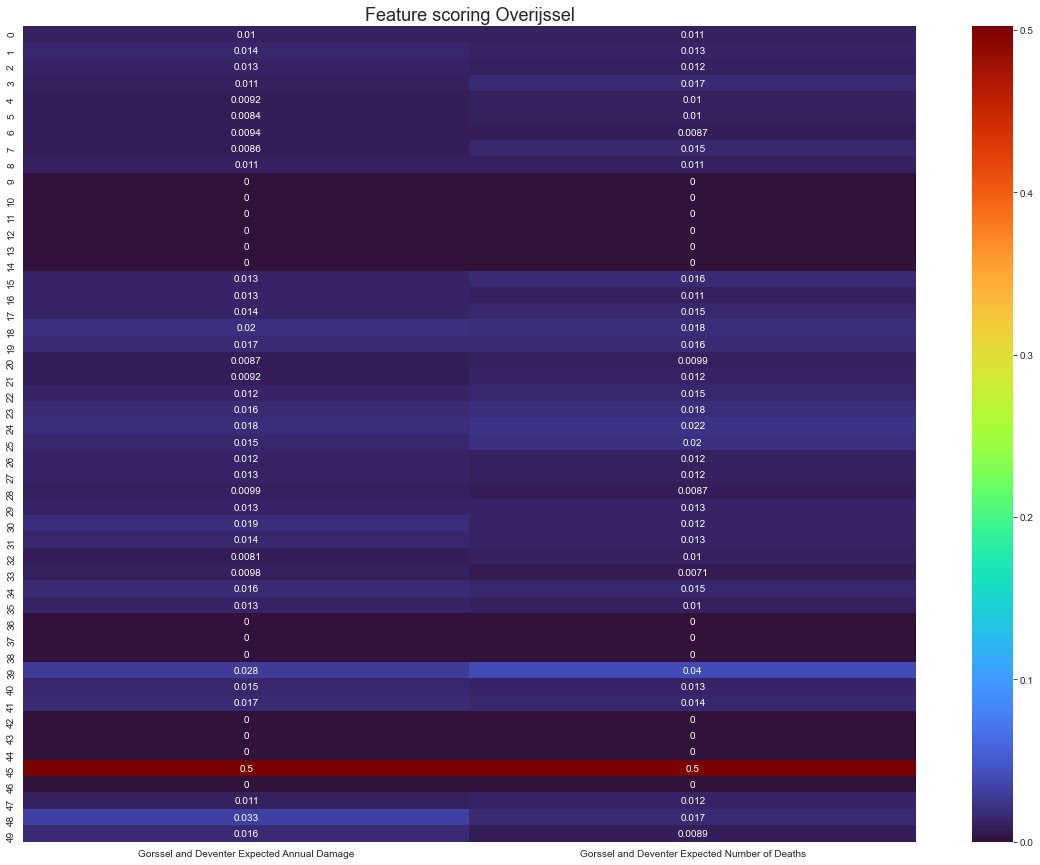
\includegraphics[width=\textwidth]{report/figures/results/sa_model_Overijssel.png}
    \caption{The results from feature scoring for the sensitivity analysis of Overijssel without policies.}
    \label{fig:feat-scor-o-wo}
\end{figure}

\begin{figure}[h!]
    \centering
    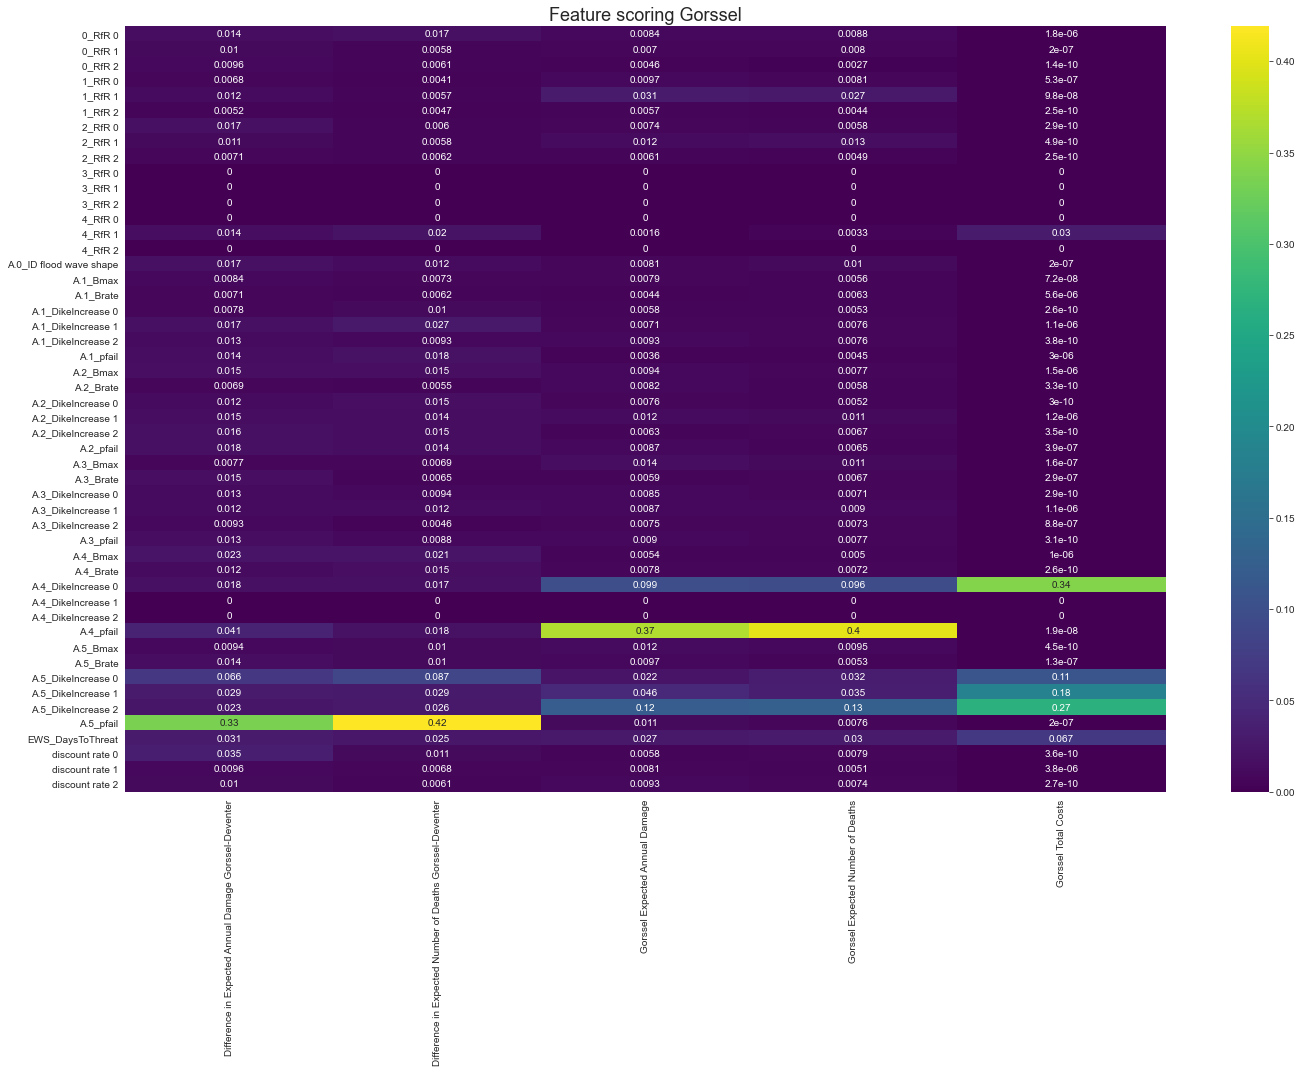
\includegraphics[width=\textwidth]{report/figures/results/Feature_scoring_Gorssel_100scen.png}
    \caption{The results from feature scoring for the sensitivity analysis of Gorssel with policies.}
    \label{fig:feat-scor-g}
\end{figure}

\begin{figure}[h!]
    \centering
    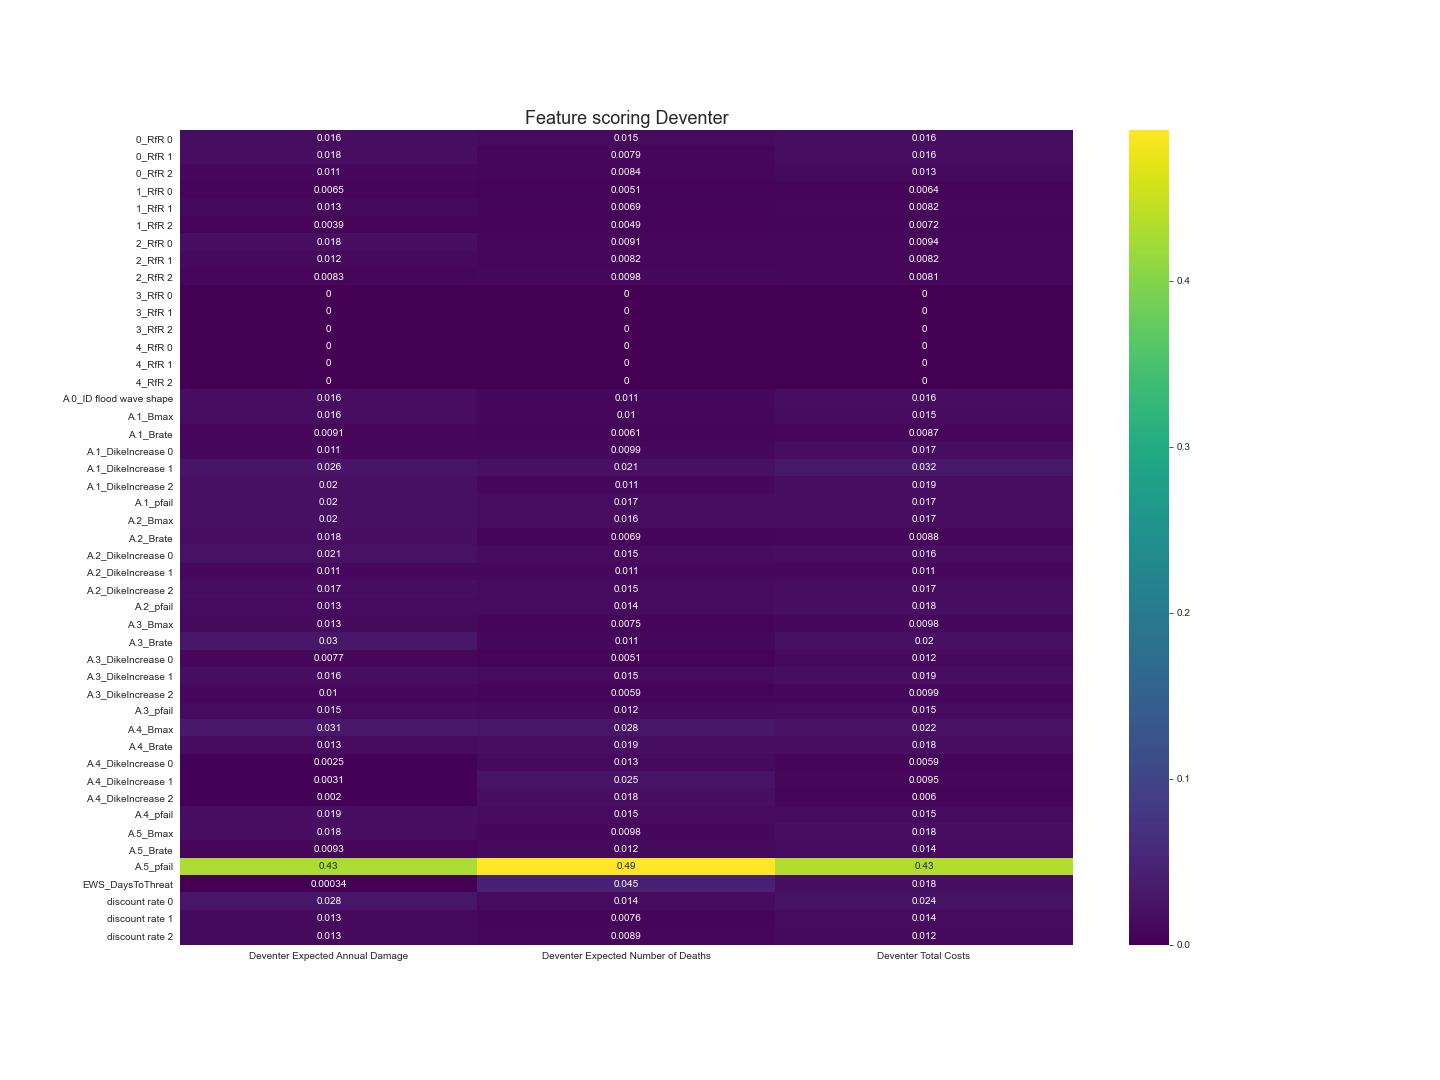
\includegraphics[width=\textwidth]{report/figures/results/Feature_scoring_Deventer_100scen.png}
    \caption{The results from feature scoring for the sensitivity analysis of Deventer with policies.}
    \label{fig:feat-scor-d}
\end{figure}

\begin{figure}[h!]
    \centering
    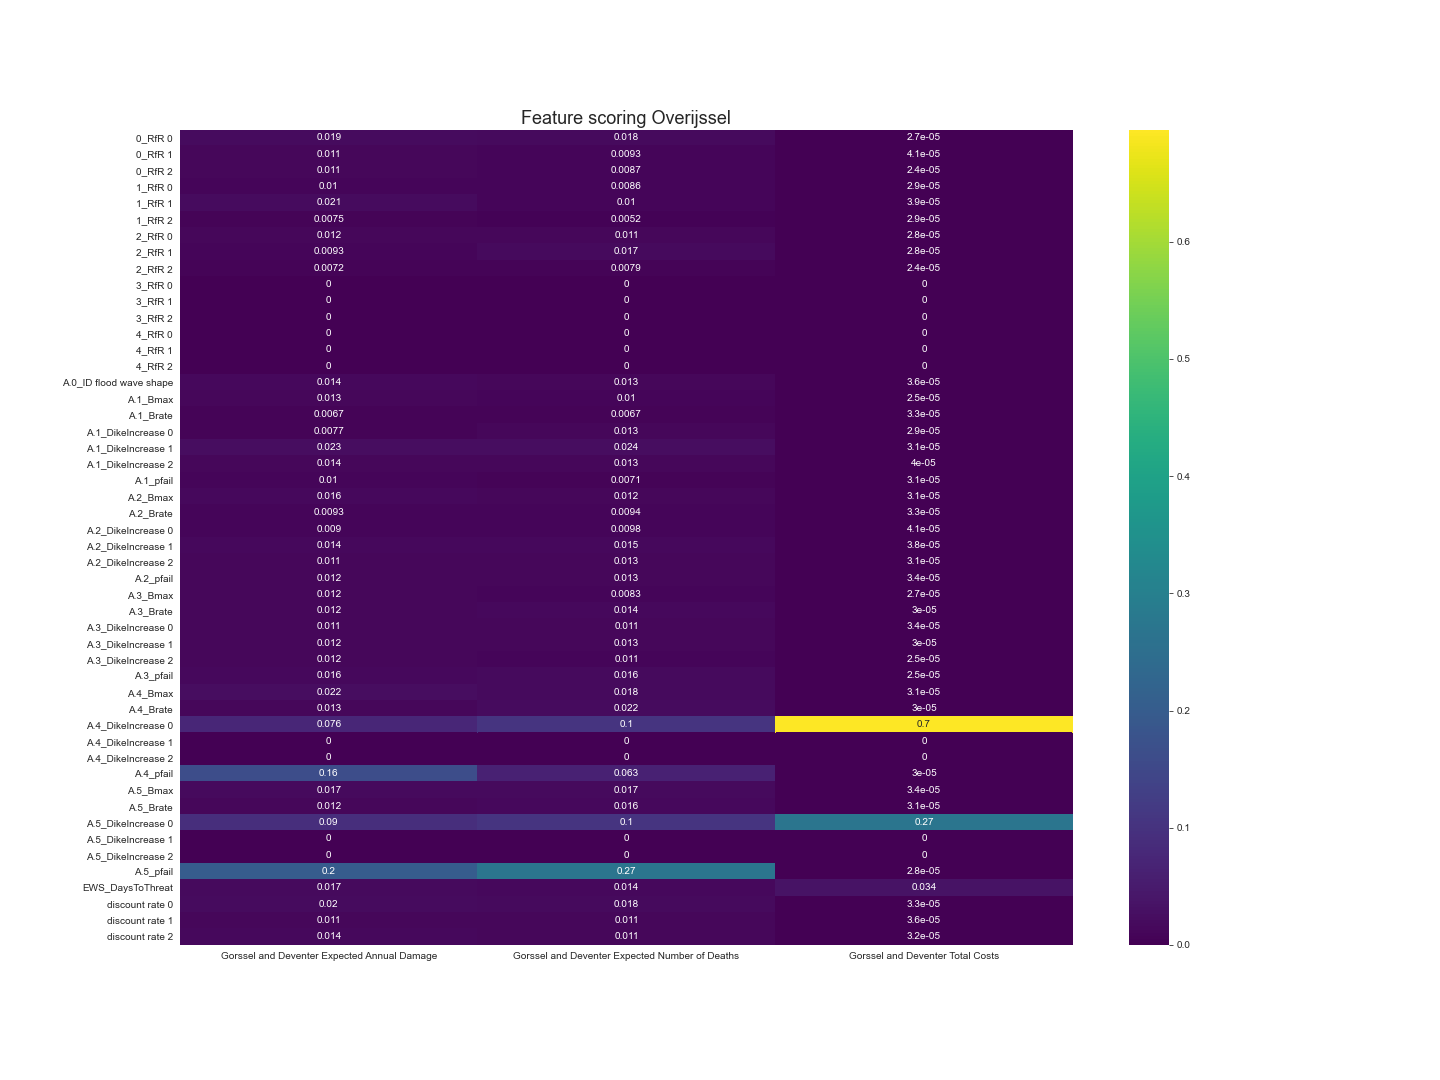
\includegraphics[width=\textwidth]{report/figures/results/Feature_scoring_Overijssel_100scen.png}
    \caption{The results from feature scoring for the sensitivity analysis of Overijssel with policies.}
    \label{fig:feat-scor-o}
\end{figure}

\newpage